\documentclass{article} % simplest latex class that gives nice default structures.  Other classes include standalone, book

% Recommended packages:
\usepackage{listings} % used for listing code

\usepackage{graphicx} % used for importing graphics

\usepackage{amsmath} % Many useful mathematical shortcuts

% Suggested packages:
\usepackage{tikz} % used for drawing figures in LaTeX directly
\usetikzlibrary{automata,calc,arrows} % some useful default tikz packages

\usepackage{enumerate} % used for finer control over enumerate lists

\usepackage{algorithm} % used for specifying algorithms
\usepackage{algpseudocode} % ditto (you need both)

\usepackage{fullpage} % reduces a page's margins to 1cm instead of 1in

\usepackage{mathpazo} % better? fonts

\usepackage{hyperref} % hyperlinks: compile with pdflatex for best results

\usepackage{amssymb}

\begin{document}


\title{\textbf{Assignment 1 COMP2022}}
\author{}
\date{}
\maketitle

\section*{Problem 1}

\subsection*{\hspace{1cm}a)}

\begin{flushleft}
\hspace{3cm}$(F \lor \bot) \equiv (\bot \lor F)$ \hspace{2cm} Commutative Law

\hspace{3cm}$(F \lor \bot) \equiv F$ \hspace{3cm} Unsatisfiability Law 
\end{flushleft}

\begin{table}[h!]
\hspace{5.5cm}
\begin{tabular}{ | c c | c | }
\hline
 $F$ & $\bot$ & $(F \lor \bot)$ \\ 
 \hline
 0 & 0 & 0 \\  
 0 & 0 & 0 \\
 1 & 0 & 1 \\
 1 & 0 & 1 \\
 \hline
\end{tabular}
\end{table}

\subsection*{\hspace{1cm}b)}

\begin{flushleft}
\hspace{2cm}$((F\lor(G\lor H)) \land (H\lor F)) \equiv (\underline{((F\lor G)\lor H)} \land (H\lor F))$ \hspace{2cm} Associative Law

\hspace{6.2cm}$\equiv (\underline{(H\lor (F\lor G))} \land (H\lor F))$ \hspace{2cm} Commutative Law

\hspace{6.2cm}$\equiv ((H\lor \underline{(G\lor F)}) \land (H\lor F))$ \hspace{2cm} Commutative Law

\hspace{6.2cm}$\equiv (\underline{(H\lor G)\lor F))} \land (H\lor F))$ \hspace{2cm} Associative Law

\hspace{6.2cm}$\equiv (\underline{(F\lor (H\lor G))} \land (H\lor F))$ \hspace{2cm} Commutative Law

\hspace{6.2cm}$\equiv ((F\lor \underline{(H\lor G)) \land F)}$ \hspace{3cm} Distributive Law

\hspace{6.2cm}$\equiv ((\underline{(F\lor H)\lor G}) \land F)$ \hspace{3cm} Associative Law

\hspace{6.2cm}$\equiv ((\underline{(H\lor F)}\lor G) \land F)$ \hspace{3cm} Commutative Law

\hspace{6.2cm}$\equiv ((H\lor F)\lor \underline{(G\land F)})$ \hspace{3cm} Associative Law

\hspace{6.2cm}$\equiv ((H\lor F)\lor \underline{(F\land G)})$ \hspace{3cm} Commutative Law

\hspace{6.2cm}$\equiv \underline{((F\land G)\lor (H\lor F))}$ \hspace{3cm} Commutative Law

\end{flushleft}

\newpage

\section*{Problem 2}

\subsection*{\hspace{1cm}a)}
\begin{flushleft}
\hspace{2cm}$G_1: (d \leftrightarrow (a \land b))$

\hspace{2cm}$G_2: (e \leftrightarrow (b \land c))$

\hspace{2cm}$G_3: (f \leftrightarrow (a \land c))$

\hspace{2cm}$G_4: (z \leftrightarrow (d \lor e \lor f))$

\hspace{2cm}$C: (z \leftrightarrow ((a \land b) \lor (b \land c) \lor (a \land c)))$
\end{flushleft}

\subsection*{\hspace{1cm}b)}
\begin{flushleft}
\hspace{2cm}$G_1: (d \leftrightarrow (c \land b))$

\hspace{2cm}$G_2: (e \leftrightarrow \neg a)$

\hspace{2cm}$G_3: (z \leftrightarrow (d \lor e))$

\hspace{2cm}$C: (z \leftrightarrow ((c \land b) \lor \neg a)$
\end{flushleft}

\newpage

\section*{Problem 3}

\subsection*{\hspace{1cm}a)}
\begin{flushleft}
\hspace{2cm}$S_1: (z \leftrightarrow (\neg(a \land b) \leftrightarrow c))$

\hspace{2cm}With the aid of truth tables, if a, b, c are all true or all false, z would be false. z is only true in

\hspace{2cm} other cases.
\end{flushleft}

\subsection*{\hspace{1cm}b)}
\begin{flushleft}
\hspace{2cm}$S_2: (z \leftrightarrow ((\neg a \leftrightarrow b) \land  c))$

\hspace{2cm}With the aid of truth tables, cases with 3 inputs or no inputs assigned true will not result in a 

\hspace{2cm}true value for z.
\end{flushleft}

\subsection*{\hspace{1cm}c)}
\begin{flushleft}
\hspace{2cm}Yes. For every circuit that implements $S_2$ to also implement $S_1$, $S_2 \models S_1$. With the aid of truth 

\hspace{2cm}tables, every row which $S_2$ is true, $S_1$ is also true ($S_2$ true in 4,6 and $S_1$ true in 2,4,6,7).
\end{flushleft}

\subsection*{\hspace{1cm}d)}
\begin{flushleft}
\hspace{2cm}Doesn't satisfy both. For the formula to satisfy $S_1$ or $S_2$, every row where formula is true 

\hspace{2cm}(rows 3,5,7), the same row for specifications also have to be true. Using a truth table, $S_1$ is true 

\hspace{2cm}in rows 2,4,6,7 and $S_2$ is true in rows 4,6, hence both doesn't meet the criteria.

\end{flushleft}

\subsection*{\hspace{1cm}e)}
\begin{flushleft}
\hspace{2cm}No. For every circuit which implements $S_1$ to also implement $S_2$, $S_1 \models S_2$. With the aid of 

\hspace{2cm}truth tables, there are rows which $S_1$ is true but $S_2$ isn't ($S_1$ true in rows 2,4,6,7, $S_2$ is true in 

\hspace{2cm}rows 4,6), the criteria is not satisfied hence $S_1$ doesn't satisfy $S_2$.
\end{flushleft}

\subsection*{\hspace{1cm}f)}
\hspace{2cm}
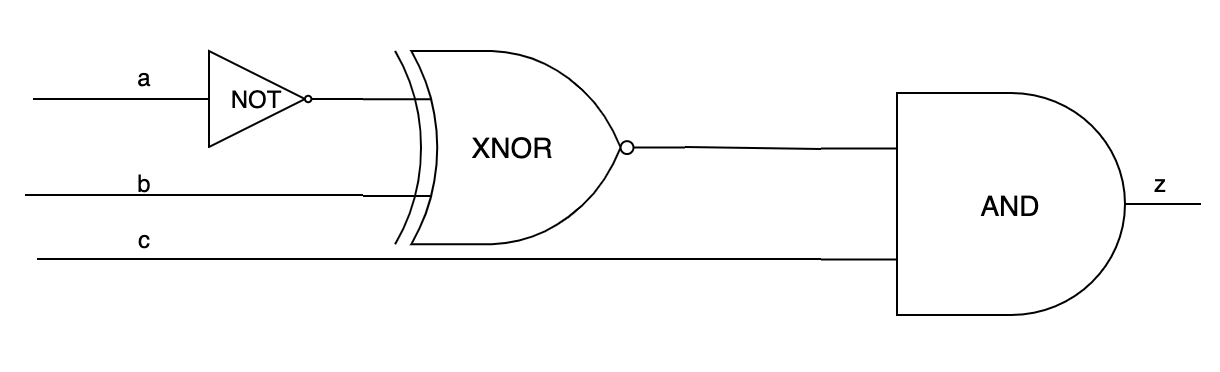
\includegraphics[width=13cm]{Circuit.png}

\subsection*{\hspace{1cm}g)}
\begin{flushleft}
\hspace{2cm}$S_c_1: (z\leftrightarrow(b \lor a) \lor c))$

\hspace{2cm}$S_c_2: (z\leftrightarrow(\neg a \lor b) \lor c))$
\end{flushleft}

\section*{Problem 4}

\subsection*{\hspace{1cm}a)}
\begin{flushleft}
\hspace{2cm}i = $a_0$ + 2$a_1$ = 1 + 2(1) = 3

\hspace{2cm}$b_3$ = 1

\hspace{2cm}M output 1.
\end{flushleft}

\subsection*{\hspace{1cm}b)}
\begin{flushleft}
\hspace{2cm}$(z\leftrightarrow ((b_0 \leftrightarrow a_0 \land a_1) \lor (b_1 \leftrightarrow a_0 \land a_1) \lor (b_2 \leftrightarrow a_0 \land a_1) \lor (b_3 \leftrightarrow a_0 \land a_1)))$
\end{flushleft}

\subsection*{\hspace{1cm}c)}
\begin{flushleft}
\hspace{2cm}\textbf{1.} $(p,q \circledcirc \bot,\bot,\bot,\top )$

\hspace{2cm}\textbf{2.} $(p,q \circledcirc \bot,p,q,\top )$

\hspace{2cm}\textbf{3.} $(p,\top \circledcirc q,p,\top,\bot )$

\hspace{2cm}\textbf{4.} $(p,q \circledcirc \top,\bot,\top,\top )$

\end{flushleft}

\end{document}
